% questions.tex —— 2004 年·全国卷Ⅳ·文科 · 题目内容片段（无答案）
% 由 tools/generate_projects.py 依来源总账自 2004/2004_数学真题_全国4文_试题.md 生成，勿手改（改源 MD 后重跑）


\begin{gktip}
\textbf{来源说明}：本题面依据固定源 PDF 两页 A3 题面逐题转录，原卷印刷页码 196–197。固定源不附答案，答案和解析均由本库独立复算。

\textbf{图形说明}：第 21 题的原卷图形关系重绘为 TikZ/PGFPlots 矢量图。图形标记所指的 PNG 不随仓库保存。
\end{gktip}

\gkpart{一、选择题（本大题共 12 小题，每小题 5 分，共 60 分．在每小题给出的四个选项中，只有一项是符合题目要求的）}

\begin{question}
\gkti{1}设集合 $U=\{0,1,2,3,4,5\}$，集合 $M=\{0,3,5\}$，$N=\{1,4,5\}$，则 $M\cap(\complement_U N)=$\mbox{（　　）}

（A）$\{5\}$　　（B）$\{0,3\}$　　（C）$\{0,2,3,5\}$　　（D）$\{0,1,3,4,5\}$

\end{question}
\begin{question}
\gkti{2}函数 $y=\mathrm{e}^{2x}$（$x\in\mathbf{R}$）的反函数为\mbox{（　　）}

（A）$y=2\ln x$（$x>0$）　　（B）$y=\ln(2x)$（$x>0$）

（C）$y=\dfrac{1}{2}\ln x$（$x>0$）　　（D）$y=\dfrac{1}{2}\ln 2x$（$x>0$）

\end{question}
\begin{question}
\gkti{3}正三棱柱侧面的一条对角线长为 2，且与底面成 $45^\circ$ 角，则此三棱柱的体积为\mbox{（　　）}

（A）$\dfrac{\sqrt{6}}{2}$　　（B）$\sqrt{6}$　　（C）$\dfrac{\sqrt{6}}{6}$　　（D）$\dfrac{\sqrt{6}}{3}$

\end{question}
\begin{question}
\gkti{4}函数 $y=(x+1)^2(x-1)$ 在 $x=1$ 处的导数等于\mbox{（　　）}

（A）1　　（B）2　　（C）3　　（D）4

\end{question}
\begin{question}
\gkti{5}为了得到函数 $y=3\times\left(\dfrac{1}{3}\right)^x$ 的图象，可以把函数 $y=\left(\dfrac{1}{3}\right)^x$ 的图象\mbox{（　　）}

（A）向左平移 3 个单位长度　　（B）向右平移 3 个单位长度

（C）向左平移 1 个单位长度　　（D）向右平移 1 个单位长度

\end{question}
\begin{question}
\gkti{6}等差数列 $\{a_n\}$ 中，$a_1+a_2+a_3=-24$，$a_{18}+a_{19}+a_{20}=78$，则此数列前 20 项和等于\mbox{（　　）}

（A）160　　（B）180　　（C）200　　（D）220

\end{question}
\begin{question}
\gkti{7}已知函数 $y=\log_{\frac{1}{4}}x$ 与 $y=kx$ 的图象有公共点 $A$，且点 $A$ 的横坐标为 2，则 $k=$\mbox{（　　）}

（A）$-\dfrac{1}{4}$　　（B）$\dfrac{1}{4}$　　（C）$-\dfrac{1}{2}$　　（D）$\dfrac{1}{2}$

\end{question}
\begin{question}
\gkti{8}已知圆 $C$ 的半径为 2，圆心在 $x$ 轴的正半轴上，直线 $3x+4y+4=0$ 与圆 $C$ 相切，则圆 $C$ 的方程为\mbox{（　　）}

（A）$x^2+y^2-2x-3=0$　　（B）$x^2+y^2+4x=0$

（C）$x^2+y^2+2x-3=0$　　（D）$x^2+y^2-4x=0$

\end{question}
\begin{question}
\gkti{9}从 5 位男教师和 4 位女教师中选出 3 位教师，派到 3 个班担任班主任（每班 1 位班主任），要求这 3 位班主任中男、女教师都要有，则不同的选派方案共有\mbox{（　　）}

（A）210 种　　（B）420 种　　（C）630 种　　（D）840 种

\end{question}
\begin{question}
\gkti{10}函数 $y=2\sin\left(\dfrac{\pi}{3}-x\right)-\cos\left(\dfrac{\pi}{6}+x\right)$（$x\in\mathbf{R}$）的最小值等于\mbox{（　　）}

（A）$-3$　　（B）$-2$　　（C）$-1$　　（D）$-\sqrt{5}$

\end{question}
\begin{question}
\gkti{11}已知球的表面积为 $20\pi$，球面上有 $A$、$B$、$C$ 三点．如果 $AB=AC=2$，$BC=2\sqrt{3}$，则球心到平面 $ABC$ 的距离为\mbox{（　　）}

（A）1　　（B）$\sqrt{2}$　　（C）$\sqrt{3}$　　（D）2

\end{question}
\begin{question}
\gkti{12}$\triangle ABC$ 中，$a$、$b$、$c$ 分别为 $\angle A$、$\angle B$、$\angle C$ 的对边．如果 $a$、$b$、$c$ 成等差数列，$\angle B=30^\circ$，$\triangle ABC$ 的面积为 $\dfrac{3}{2}$，那么 $b=$\mbox{（　　）}

（A）$\dfrac{1+\sqrt{3}}{2}$　　（B）$1+\sqrt{3}$　　（C）$\dfrac{2+\sqrt{3}}{2}$　　（D）$2+\sqrt{3}$

\end{question}
\gkpart{二、填空题（本大题共 4 小题，每小题 4 分，共 16 分．把答案填在横线上）}

\begin{question}
\gkti{13}$\left(x-\dfrac{1}{\sqrt{x}}\right)^8$ 展开式中 $x^5$ 的系数为 $\underline{\hspace{3cm}}$．

\end{question}
\begin{question}
\gkti{14}已知函数 $y=\dfrac{1}{2}\sin\dfrac{x+\pi}{A}$（$A>0$）的最小正周期为 $3\pi$，则 $A=\underline{\hspace{3cm}}$．

\end{question}
\begin{question}
\gkti{15}向量 $\vec{a}$、$\vec{b}$ 满足 $(\vec{a}-\vec{b})\cdot(2\vec{a}+\vec{b})=-4$，且 $|\vec{a}|=2$，$|\vec{b}|=4$，则 $\vec{a}$ 与 $\vec{b}$ 夹角的余弦值等于 $\underline{\hspace{3cm}}$．

\end{question}
\begin{question}
\gkti{16}设 $x,y$ 满足约束条件：
\nopagebreak[4]
\[
\begin{cases}
x+y\leqslant 1,\\
y\leqslant x,\\
y\geqslant 0,
\end{cases}
\]
则 $z=2x+y$ 的最大值是 $\underline{\hspace{3cm}}$．

\end{question}
\gkpart{三、解答题（本大题共 6 小题，共 74 分．解答应写出文字说明、证明过程或演算步骤）}

\begin{question}
\gkti{17}（本小题满分 12 分）

已知 $\alpha$ 为第二象限角，且 $\sin\alpha=\dfrac{\sqrt{15}}{4}$，求 $\dfrac{\sin\left(\alpha+\dfrac{\pi}{4}\right)}{\sin 2\alpha+\cos 2\alpha+1}$ 的值．

\end{question}
\begin{question}
\gkti{18}（本小题满分 12 分）

已知数列 $\{a_n\}$ 为等比数列，$a_2=6$，$a_5=162$．

（1）求数列 $\{a_n\}$ 的通项公式；

（2）设 $S_n$ 是数列 $\{a_n\}$ 的前 $n$ 项和，证明 $\dfrac{S_n\cdot S_{n+2}}{S_{n+1}^2}\leqslant 1$．

\end{question}
\begin{question}
\gkti{19}（本小题满分 12 分）

已知直线 $l_1$ 为曲线 $y=x^2+x-2$ 在点 $(1,0)$ 处的切线，$l_2$ 为该曲线的另一条切线，且 $l_1\perp l_2$．

（1）求直线 $l_2$ 的方程；

（2）求由直线 $l_1$、$l_2$ 和 $x$ 轴所围成的三角形的面积．

\end{question}
\begin{question}
\gkti{20}（本小题满分 12 分）

某同学参加科普知识竞赛，需回答 3 个问题．竞赛规则规定：答对第一、二、三问题分别得 100 分、100 分、200 分，答错得零分．假设这名同学答对第一、二、三个问题的概率分别为 0.8、0.7、0.6，且各题答对与否相互之间没有影响．

（1）求这名同学得 300 分的概率；

（2）求这名同学至少得 300 分的概率．

\Needspace{0.4\textheight}
\end{question}
\begin{question}
\gkti{21}（本小题满分 12 分）

如图，四棱锥 $P-ABCD$ 中，底面 $ABCD$ 为矩形，$AB=8$，$AD=4\sqrt{3}$，侧面 $PAD$ 为等边三角形，并且与底面所成二面角为 $60^\circ$．
\nopagebreak[4]
\begin{center}% 2004 年全国卷Ⅳ文科第 21 题：四棱锥立体几何图
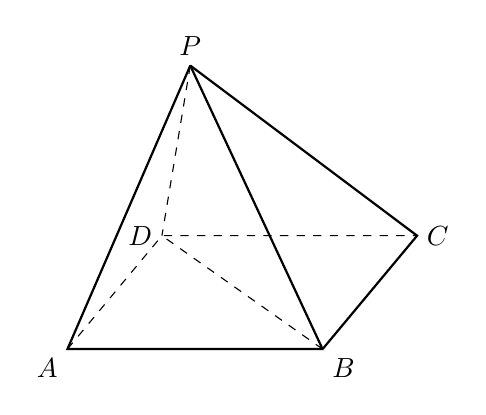
\begin{tikzpicture}[>=stealth,scale=1.2]
  % Coordinates
  \coordinate (A) at (-1.5,-0.8);
  \coordinate (B) at (1.2,-0.8);
  \coordinate (C) at (2.2,0.4);
  \coordinate (D) at (-0.5,0.4);
  \coordinate (P) at (-0.2,2.2);

  % Solid edges
  \draw[thick] (P) -- (A) -- (B) -- (C) -- (P);
  \draw[thick] (P) -- (B);

  % Dashed edges
  \draw[dashed] (A) -- (D) -- (C);
  \draw[dashed] (P) -- (D);
  \draw[dashed] (B) -- (D);

  % Labels
  \node[below left] at (A) {$A$};
  \node[below right] at (B) {$B$};
  \node[right] at (C) {$C$};
  \node[left] at (D) {$D$};
  \node[above] at (P) {$P$};
\end{tikzpicture}
\end{center}
\nopagebreak[4]
（1）求四棱锥 $P-ABCD$ 的体积；

（2）证明：$PA\perp BD$．

\end{question}
\begin{question}
\gkti{22}（本小题满分 14 分）

双曲线 $\dfrac{x^2}{a^2}-\dfrac{y^2}{b^2}=1$（$a>1,b>0$）的焦点距为 $2c$，直线 $l$ 过点 $(a,0)$ 和 $(0,b)$，且点 $(1,0)$ 到直线 $l$ 的距离与点 $(-1,0)$ 到直线 $l$ 的距离之和 $s\geqslant\dfrac{4}{5}c$．求双曲线的离心率 $e$ 的取值范围．

\end{question}